\chapter{Name of chapter 3}
\setcounter{secnumdepth}{3}
\label{chap:chap3}
\section{Overview}

Orthogonal frequency Division Multiplexing (OFDM) employs Multi-Carrier Modulation (MCM) technique highly attractive for implementation and received considerable attention due to the need for high speed data transmission. Orthogonal sub carriers allow their spectrums to overlap which achieves the high spectral efficiency.



\section{Hyperparameter Tunning-Improving neural networks}
Building a Deep neural network architecture for a specific application it is not a big issue. To reduce the time needed for training deep neural network model and for improving its accuracy we have to use hyperparameter tuning. These techniques are very useful for reducing training period. This section divided into three parts i.e first part will explain how to divide the data into training set, development set, test set and it covers some regularization techniques, dropout methods, batch normalisation process etc. Part 2 will give brief idea about optimizers that is RMSprop and Adam optimizer. Finally we can see how hyperparameter tuning can improve the model efficiency. Choosing hyperparameters and observing their effect on efficiency it is very crucial part in training neural networks. There is no standardized way for choosing hyperparameters. We can select hyperparameters according to the results given by tuning this is completely observation process.\\
\par Some of the hyper parameters are listed below 
\begin{itemize}
    \item Different types of active functions used at input, hidden  and output layers. 
    \item  Learning rate 
    \item How many hidden layers and how many units present in each hidden layer.
\end{itemize}


\subsection{Bias and Variance}
If we are classifying objects using a straight line then and it is called under-fit and it is highly biased. If we will classify the objects perfectly using curves then it is called over-fit and that are high variance. 

\begin{figure}
    \centering
    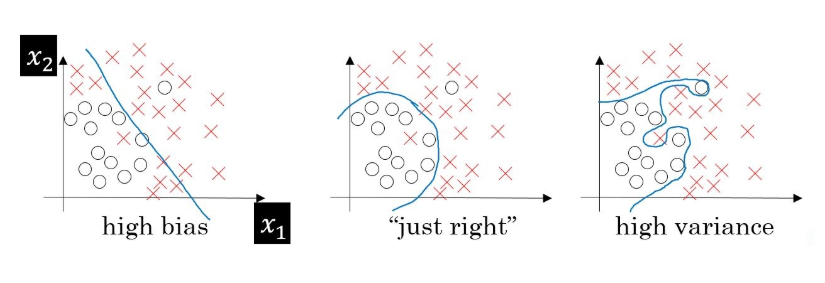
\includegraphics[width=15cm,,scale=5]{Screenshot (137).png}
    \caption{ Curves for showing under fit and over fit data \cite{jain} }
    \label{fig:my_label}
\end{figure}

For best model always bias and variance values should be less. Choosing the best model includes checking the training set and testing set error. 
some points to keep in mind for choosing the model 


\begin{itemize}
    \item If test set error is greater than train set error then model representing over fitting and it has high variance.
    \item If test set and train set error both are having high value then model represented as underfitting and it has high bias.
    \item  If Training set error is more than test set error then model has high variance and high bias. 
    \item  Train set and test set error both are small then data is fitted reasonably, Hence model as low variance and low bias.
\end{itemize}




\begin{center}
     ***
 \end{center}



